%%% Exemple of presentation using LaTeX-beamer theme for GI
%%% (c) Pierre Lemaire, 2015, 2016.
%%% Released under license CC-BY-SA 4.0 (https://creativecommons.org/licenses/by-sa/4.0/)
%%% Logos and images may be copyrighted. 

\documentclass[colors]{beamer}
\setbeameroption{hide notes}

\usepackage[T1]{fontenc}
\usepackage[utf8]{inputenc}
\usepackage{amsbsy} % bold math symbols

\usetheme{GI}

\def\blankframe{\frame<0|handout:1>{\thispagestyle{empty}\addtocounter{framenumber}{-1}}}
\def\epsilon{\varepsilon}
\long\def\TODO#1{}
\long\def\IGNORE#1{}

% === document info ===========================================================
\title[ADGI]{Analyse de données pour le génie industriel}
\subtitle{Régression linéaire simple}
\author[Joly, Lemaire]{Iragaël Joly \and Pierre Lemaire}%
\institute{Grenoble INP -- Génie Industriel, 2A}%
\date{2015--2016}%
\subject{analyse de données}
\keywords{analyse de données}

\begin{document}

%% =============================================================================
\frame{%
  \frametitle{Bibliographie}

  \begin{thebibliography}{99}
  \bibitem{} P.-A. Cornillon et al. \textit{Statistiques avec R}, PU
    Rennes, 2012.
  \bibitem{} S. Tufféry. \textit{Data Mining et statistique
      décisionnelle}, Technip, 2012.
  \bibitem{} G. Saporta. \textit{Probabilités et analyse de données},
    Technip, 2011.
  \end{thebibliography}
}

%% =============================================================================
%% =============================================================================
\section[Régression linéaire]{Régression linéaire simple}
\subsection{Définitions et calculs}

% -----------------------------------------------------------------------------
\frame[allowframebreaks]{%
  \frametitle{Régression}
  \begin{itemize}
  \item les données sont une matrice $n \times (p+1)$
    \begin{itemize}
    \item un échantillon de $n$ \alert{observations}
    \item chaque observation est constituée de $p+1$ variables
    \item une \alert{réponse} (ou variable dépendante ou à
      expliquer)~: $y$
    \item des \alert{variables explicatives} (ou indépendantes)~:
      $x_1, x_2, ..., x_{p}$
    \end{itemize}
    
    \[\scriptsize\left(\begin{array}{l|llll}
      y_1 & x_{11} & x_{21} & \ldots & x_{p1} \\
      y_2 & x_{12} & x_{22} & \ldots & x_{p2} \\
      \vdots &    &       &        & \vdots\\
      y_n & x_{1n} & x_{2n} & \ldots & x_{pn} \\
      \end{array}\right)\]

    \nobreak

  %\item %définition
    \begin{block}{Régression}
      une régression de $y$ sur $\mathbf{x}$ est un modèle de la
      forme \[ y = f(\mathbf{x}) + \epsilon\]
    \end{block}
    \begin{itemize}
    \item $f$ caractérise l'effet de $\mathbf{x}$ sur $y$~; la forme
      de $f$ est une \alert{hypothèse}
    \item $\varepsilon$ représente l'effet des autres facteurs (non
      pris en compte)
    \end{itemize}

  \end{itemize}
}


% -----------------------------------------------------------------------------
\frame{%
  \frametitle{Erreurs de régression}
  
  \noindent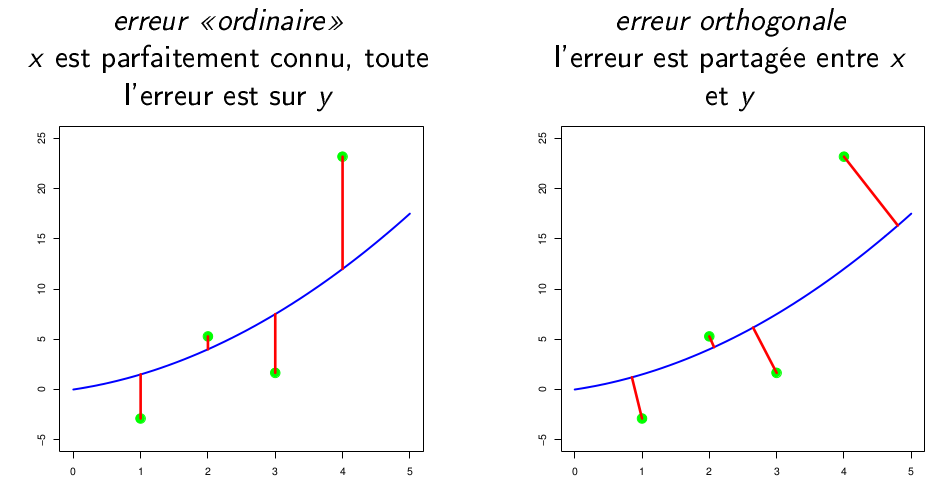
\includegraphics[width=\textwidth]{Img/reglin_erreur}
  \begin{itemize}
  \item[]\begin{itemize}
    \item modèle $y = f(x) + \epsilon$ implique une \alert{erreur
        ordinaire}
    \item l'erreur ordinaire est une \alert{hypothèse} à valider
      %% on maîtrise bien x (plan d'expériences)
      %% les calculs sont plus simples
    \end{itemize}
  \end{itemize}
}

% -----------------------------------------------------------------------------
\frame{%
  \frametitle{Agrégation des erreurs de régression}
  \begin{itemize}
  \item enjeu~: minimiser les erreurs, donc la norme de $\epsilon$

    \vfill
  \item norme $L_1$~: $||\epsilon||_1 = \sum_{i=1}^n|\epsilon_i|$
    \begin{itemize}
    \item poids des erreurs proportionnel à la valeur
    \item non dérivable en zéro, donc peu adaptée à l'optimisation
    \end{itemize}

    \smallskip
  \item norme $L_2$~: $||\epsilon||_2 = \sqrt{\sum_{i=1}^n\epsilon_i^2}$
    \begin{itemize}
    \item privilégie plusieurs petites erreurs à une grosse
    \item très bien adaptée à l'optimisation
    \item «\alert{moindres carrés}»
    \end{itemize}

    \smallskip
  \item norme $L_{\infty}$~: $||\epsilon||_{\infty} = \max_{i=1}^n|\epsilon_i|$
    \begin{itemize}
    \item erreur «égale» pour tous (idéalement), contrôle du pire cas
    \item peu adaptée à l'optimisation
    \end{itemize}

    \vfill
  \item \alert{nous nous restreindrons aux moindres carrés ordinaires}
  \end{itemize}
  % 
}

% -----------------------------------------------------------------------------
\frame{%
  \frametitle{Régression linéaire simple (1)}
  \begin{itemize}
  \item on se limite à une unique variable explicative $x$
  \item on se limite à une fonction linéaire

    \vfill
    \begin{block}{Régression linéaire simple}% Gaudoin, p8
      Le modèle de régression linéaire simple est défini par
      \[ y_i = \beta_1 x_i + \beta_0 + \epsilon_i, i=1..n\]
    \end{block}
    \begin{itemize}
    \item $\beta_1$ et $\beta_0$ sont les paramètres inconnus à estimer
    \item $\epsilon_i$ est l'erreur ou \alert{résidu} pour l'observation $i$
    \end{itemize}
    \vfill
  \end{itemize}
}

% -----------------------------------------------------------------------------
\frame{%
  \frametitle{Régression linéaire simple (2)}
  \begin{itemize}
  \item d'un point de vue statistique (deuxième partie du cours)~:
    \begin{itemize}
    \item $y_i$ est la réalisation d'une variable aléatoire $Y_i$
    \item il y a des hypothèses fortes sur les résidus~: \\
      \alert{indépendants}, \alert{de même loi}, \alert{centrés} et
      \alert{de même variance $\sigma^2$}
      \begin{itemize}
      \item le modèle donne la valeur \emph{moyenne} de $Y$~: \\
        $E[Y_i] = E[\beta_1 x_i + \beta_0 + \epsilon_i] = \beta_1 x_i
        + \beta_0$
      \item $\sigma^2$ représente le bruit ou poids des autres facteurs~: \\
        $var[Y_i] = var[\beta_1 x_i + \beta_0 + \epsilon_i] =
        \sigma^2$
      \end{itemize}
    \end{itemize}

    \vfill

  \item enjeux~:
    \begin{itemize}
    \item estimer $\beta_1$ et $\beta_0$~; faire des tests
      d'hypothèses sur ces paramètres 
    \item faire des tests d'hypothèses sur la validité du modèle, sur
      les prédictions
    \end{itemize}

  \end{itemize}
}


% -----------------------------------------------------------------------------
\frame{%
  \frametitle{Calcul de $\beta_1$ et $\beta_0$}% Gaudoin, p15
  \begin{itemize}
  \item on veut minimiser l'erreur quadratique (moyenne)~: \[\delta^2
    =
    \frac{1}{n}\sum_{i=1}^n\epsilon_i^2 = \frac{1}{n}\sum_{i=1}^n(y_i
    - \beta_1 x_i - \beta_0)^2\]

    \vfill
  \item\null[... quelques calculs ...]
    \vfill
  \end{itemize}
}

% -----------------------------------------------------------------------------
\frame{%
  \frametitle{Droite des moindres carrés}
  \begin{itemize}
  \item[]
    \begin{block}{Droite des moindres carrés}
      La droite des moindres carrées est $y = \beta_1 x + \beta_0$
      avec
      \[%
      \beta_1 = \frac{C_{xy}}{s^2_x}
      \kern2cm%
      \beta_0 = \bar{y} - \beta_1\bar{x}%
      \]
    \end{block}
    \begin{itemize}\scriptsize
    \item $\bar{x} = \frac{1}{n}\sum_{i=1}^nx_i$ \hfill(moyenne de $x$)
    \item $\bar{y} = \frac{1}{n}\sum_{i=1}^ny_i$ \hfill(moyenne de $y$)
    \item $s^2_x = \frac{1}{n}\sum_{i=1}^n(x_i -\bar{x})^2 =
      \frac{1}{n}\sum_{i=1}^nx_i^2 - \bar{x}^2$ \hfill(variance de $x$)
    \item $C_{xy} = \frac{1}{n}\sum_{i=1}^n(x_i -\bar{x})(y_i -
      \bar{y}) = \frac{1}{n}\sum_{i=1}^nx_iy_i - \bar{x}\bar{y}$
      \hfill(covar. entre $x$ et $y$)
      \vfill
    \item $\beta_1$ et $\beta_0$ sont estimateurs sans biais des
      variables aléatoires correspondantes
    \end{itemize}
    \vfill
  \item $y = \bar{y} - \frac{C_{xy}}{s^2_x}(x - \bar{x})$
  \item la droite passe par le barycentre $(\bar{x};\bar{y})$
  \end{itemize}
}

%% =============================================================================
\subsection{Travaux pratiques}
% -----------------------------------------------------------------------------
\frame{%
  \frametitle{TP~: Échauffement}
  
  \begin{enumerate}
  \item Générez $\mathtt{x} = (1;2;\ldots;100)$ et $\mathtt{y}$ de la
    forme $y = f(x) + \epsilon$
    % pour $f$ et $\epsilon$ de votre choix.
    \\ on prendra $y = 0.05 x^2 - 3 x + 7 + {\cal N}(\mu=0,\sigma=50)$

    % f : modèle, par exemple linéaire... ou pas ; \epsilon : erreur

    \bigskip
  \item Tracez $\mathtt{y}$ en fonction de $\mathtt{x}$~; donnez un
    nom aux axes et au graphique. % Vérifiez que $\mathtt{y}$ n'est pas
    % «trop» linéaire en $\mathtt{x}$.

    \bigskip
  \item Calculez la variance de $\mathtt{x}$ et la covariance de
    $\mathtt{x}$ et $\mathtt{y}$ (faire vos propres
    fonctions). Comparez aux résultats des fonctions \texttt{var} et
    \texttt{cov}.

    \bigskip
  \item \emph{Astuce}~: savez-vous afficher la valeur de la variance
    de $\mathtt{x}$ avec exactement 3 décimales (\texttt{sprintf})~?
  \end{enumerate}
}

% -----------------------------------------------------------------------------
\frame{%
  \frametitle{TP~: Calculs de base}
  \begin{enumerate}
  \item Calculez $\beta_1$ et $\beta_0$ (faire des fonctions)

    \bigskip
  \item Définissez deux fonctions qui permettent respectivement de
    calculer une régression linéaire et de l'évaluer sur des nouvelles
    données.

    \bigskip
  \item Calculez la régression linéaire de $\mathtt{y}$ en fonction de
    $\mathtt{x}$

    \bigskip
  \item Ajoutez la droite de régression sur le graphique %de
    % $\mathtt{y}$ en fonction de $\mathtt{x}$
    (\texttt{abline}).

    \bigskip
  \item \emph{Astuce}~: savez-vous modifier la couleur, l'épaisseur ou
    le style d'un tracé (\texttt{col}, \texttt{lwd}, \texttt{lty})~?

  \end{enumerate}
}

% -----------------------------------------------------------------------------
\frame{%
  \frametitle{TP~: Calculs des erreurs}
  \begin{enumerate}
  \item Calculez le vecteur des erreurs.

    \bigskip
  \item Calculez l'erreur quadratique moyenne. Calculez l'erreur
    moyenne, l'erreur absolue moyenne, l'erreur relative moyenne,
    l'erreur relative absolue moyenne. 

    \bigskip
  \item Déterminez pour combien et pour quelles valeurs de \texttt{x}
    l'erreur absolue est plus grande que 100.
    
    \bigskip
  \item Tracez la courbe $N(e)$ où $N(e)$ représente le nombre de
    valeurs de valeurs de $\mathtt{x}$ pour lesquelles l'erreur est
    supérieure à $e$.

    \bigskip
  \item \emph{Astuce}~: connaissez-vous \texttt{sapply}~?
  \end{enumerate}
}

%% =============================================================================
%% =============================================================================
\section[Qualité d'une rég.]{Qualité d'une régression}
\subsection{Évaluation de la qualité d'une régression}

% -----------------------------------------------------------------------------
\frame{%
  \frametitle{Évaluation empirique des erreurs}
  $y$~: vecteur des valeurs mesurées~; $\hat{y}$~: vecteur des valeurs prédites
  \vfill
  \begin{itemize}
  \item somme des erreurs quadratiques~: $\sum_i(y_i - \hat{y}_i)^2$ (norme $L2$)\\
    (moindres carrés)
  \item somme des erreurs absolues~:  $\sum_i|y_i - \hat{y}_i|$ 
    (norme $L1$)
  \item plus grande erreur absolue~: $\max_i|y_i - \hat{y}_i|$ (norme $L_{\infty}$)

    \vfill

  \item somme des erreurs relatives~: $\sum_i\left|\frac{y_i -
        \hat{y}_i}{y_i}\right|$

  \item plus grande erreur relative~: $\max_i\left|\frac{y_i -
        \hat{y}_i}{y_i}\right|$
    
    \vfill
    
  \item ...
  \end{itemize}

}

% -----------------------------------------------------------------------------
\frame{%
  \frametitle{Coefficient de corrélation linéaire}
  \begin{itemize}
  \item[]
    \begin{block}{Coefficient de corrélation}
      Le coefficient de corrélation linéaire (empirique) entre les
      $x_i$ et les $y_i$ est \[r_{xy} = \frac{C_{xy}}{s_xs_y}\]
      \scriptsize où $C_{xy}$ est la covariance entre $x$ et $y$,
      $s_x$ et $s_y$ sont les écarts-types de $x$ et $y$
    \end{block}
    
    \vfill
  \item $\delta^2 = s_y^2(1-r^2_{xy})$~: minimiser $\delta$ est
    équivalent à maximiser $r^2_{xy}$ % Gaudoin, p16
  \item $r_{xy} =\pm 1$ ssi les points sont parfaitements alignés
  \item $r_{xy} \in [-1;1]$ % car l'erreur est plus petite que la variance sur y
  \end{itemize}
}

% -----------------------------------------------------------------------------
\frame{%
  \frametitle{Décomposition de la variance}% Tuffery, p427 + Gaudoin p25, Joly p41
  \begin{itemize}
  \item Soit $\hat{y}_i = \beta_1 x_i + \beta_0$, et donc $y_i =
    \hat{y}_i+\epsilon_i$
  \item On peut décomposer la variance~:
    $\underbrace{y_i - \bar{y}}_{\hbox{variance}} %
    = \underbrace{\hat{y}_i - \bar{y}}_{\hbox{expliquée}}%
    + \underbrace{\epsilon_i}_{\hbox{non expliquée}}$

    \vfill
    
  \item on appelle \alert{variance totale} $SST =
    \frac{1}{n}\sum_{i=1}^n(y_i - \bar{y})^2$
    
  \item on appelle \alert{variance expliquée} $SSE =
    \frac{1}{n}\sum_{i=1}^n(\hat{y}_i - \bar{y})^2$

  \item on appelle \alert{variance résiduelle} $SSR =
    \frac{1}{n}\sum_{i=1}^n(y_i - \hat{y}_i)^2 = \delta_{\min}^2$

    \begin{block}{Décomposition de la variance}
      \[SST = SSE + SSR\]
    \end{block}
    % \begin{itemize}\scriptsize
    % \item admis % ... démonstration dans Gaudoin, p25-26
    % \end{itemize}
  \end{itemize}
}

% -----------------------------------------------------------------------------
\frame[allowframebreaks]{%
  \frametitle{Coefficient de détermination}% Tuffery, p427 + Gaudoin p25, Joly p41
  \begin{itemize}
  \item[]
    \begin{block}{Coefficient de détermination}
      Le coefficient de détermination de la régression linéaire
      est \[R^2 = \frac{SSE}{SST} = 1 - \frac{SSR}{SST}\]
    \end{block}\kern-5mm
  \item $R^2$ est la proportion de la variance de $y$ expliquée par $x$
    \begin{itemize}
    \item $R^2$ proche de 1~: $x$ et $y$ \emph{semblent} en relation linéaire
    \item $R^2$ proche de 0~: $x$ et $y$ ne sont pas liés \emph{linéairement}
    \end{itemize}

  \item propriété~: $R^2 = r_{xy}^2$
  \end{itemize}
  
  
  \hfill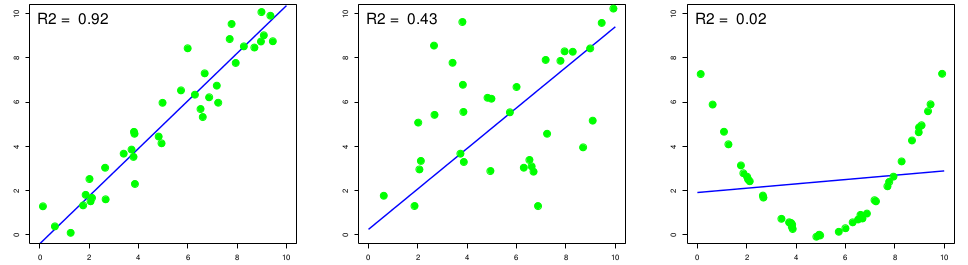
\includegraphics[width=\textwidth]{Img/reglin_coefdet}\hfill\null
}

% -----------------------------------------------------------------------------
\frame{%
  \frametitle{Analyse des résidus}% 
  \begin{itemize}
  \item résidus en fonction de $x$ (ou $y$ ou $\hat{y}$)
  \end{itemize}
  \noindent\kern-3mm
  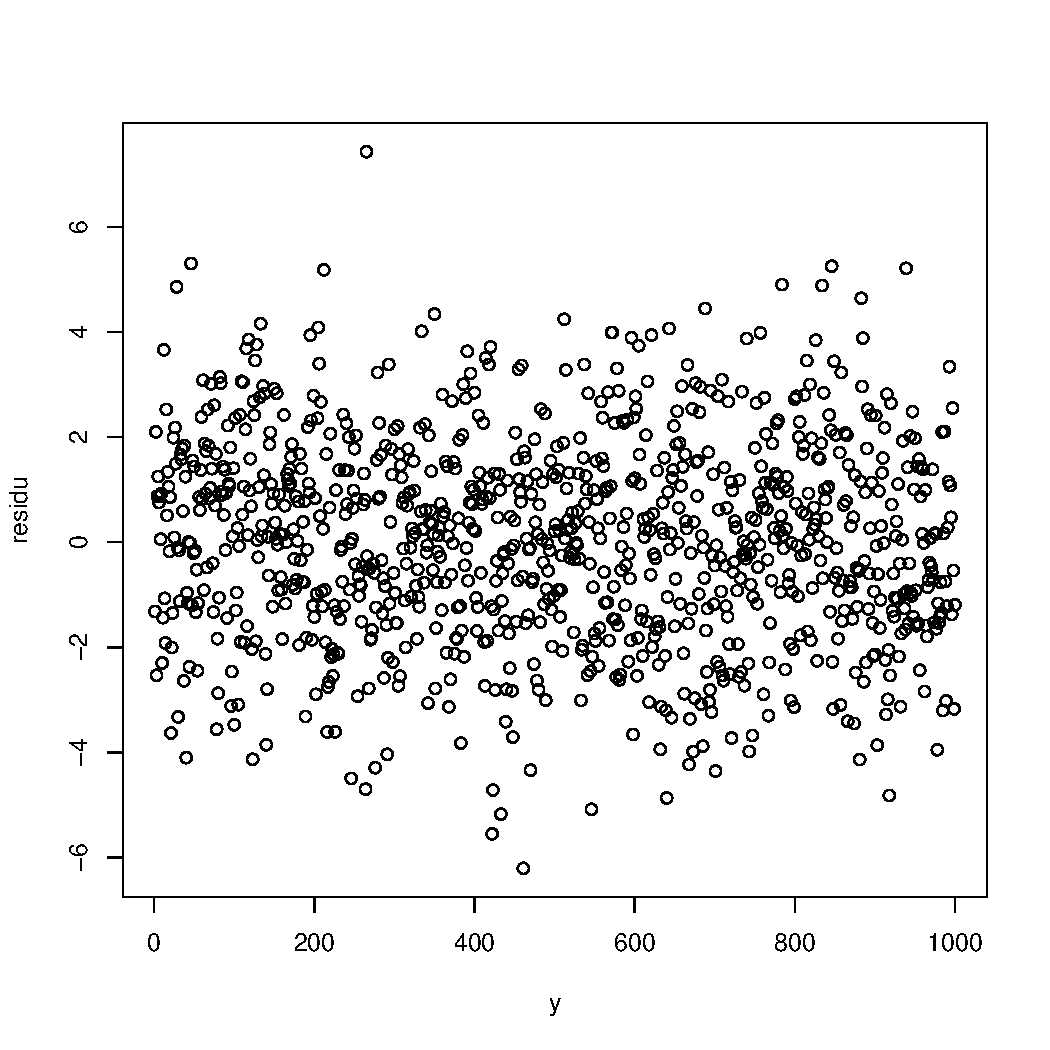
\includegraphics[width=.36\textwidth]{Img/reglin_residu_1}%
  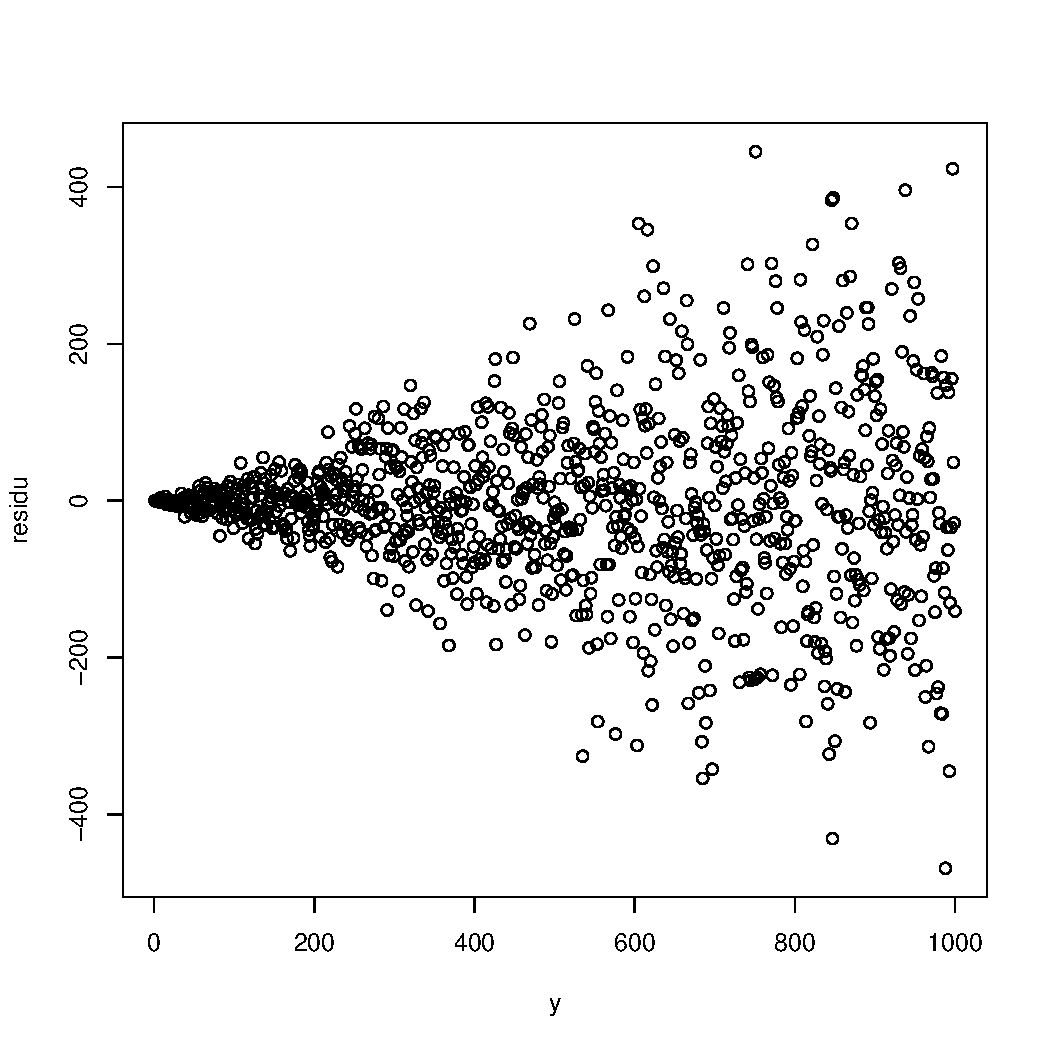
\includegraphics[width=.36\textwidth]{Img/reglin_residu_2}%
  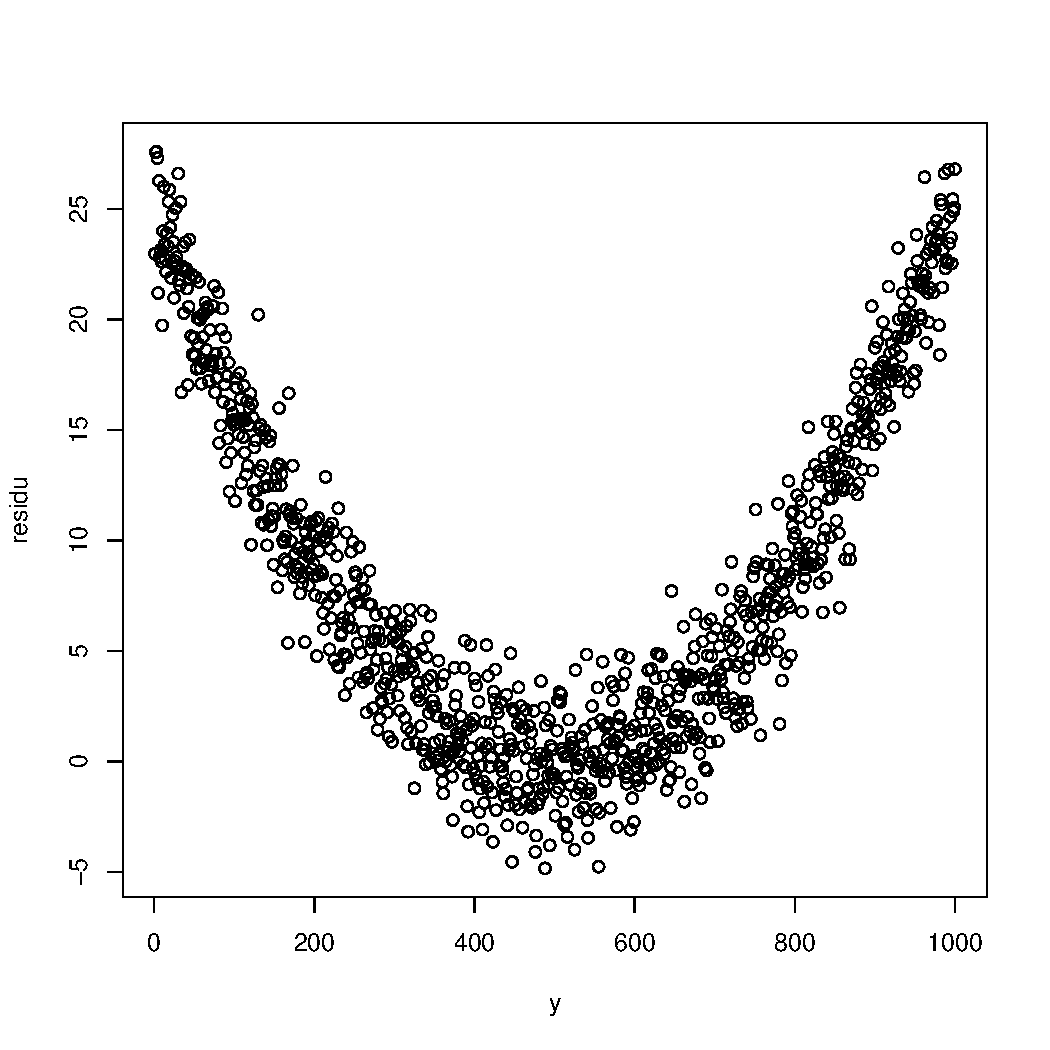
\includegraphics[width=.36\textwidth]{Img/reglin_residu_3}

  \noindent\kern-3mm
  \hbox to .36\textwidth{\hfill normal\hfill}%
  \hbox to .36\textwidth{\hfill hétéroscédasticité\hfill}%
  \hbox to .36\textwidth{\hfill composante\hfill}%
  
  \noindent\kern-3mm\kern .72\textwidth%
  \hbox to .36\textwidth{\hfill non linéaire\hfill}%
  
  \IGNORE{
    xs <- 1:1000
    ys <- rnorm(n=length(xs), mean=0, sd=2)
    pdf("reglin_residu_1.pdf")
    plot(xs,ys, xlab="y", ylab="residu")
    dev.off()

    pdf("reglin_residu_2.pdf")
    ys <- rnorm(n=length(xs), mean=0, sd=2)*xs/10
    plot(xs,ys, xlab="y", ylab="residu")
    dev.off()

    pdf("reglin_residu_3.pdf")
    ys <- rnorm(n=length(xs), mean=0, sd=2) + 0.0001*(xs-max(xs)/2)^2
    plot(xs,ys, xlab="y", ylab="residu")
    dev.off()

    xs <- 1:100
    ys <- rnorm(n=length(xs), mean=0, sd=2)
    pdf("reglin_residu_out.pdf")
    plot(xs,ys, xlab="y", ylab="residu")
    abline(h=c(-3,-2,0,2,3), lty=c(3,2,1,2,3), lw=2, col=c("green", "orange", "red", "orange", "green"))
    dev.off()
  }
}

% -----------------------------------------------------------------------------
\frame{%
  \frametitle{Observations suspicieuses}% 
  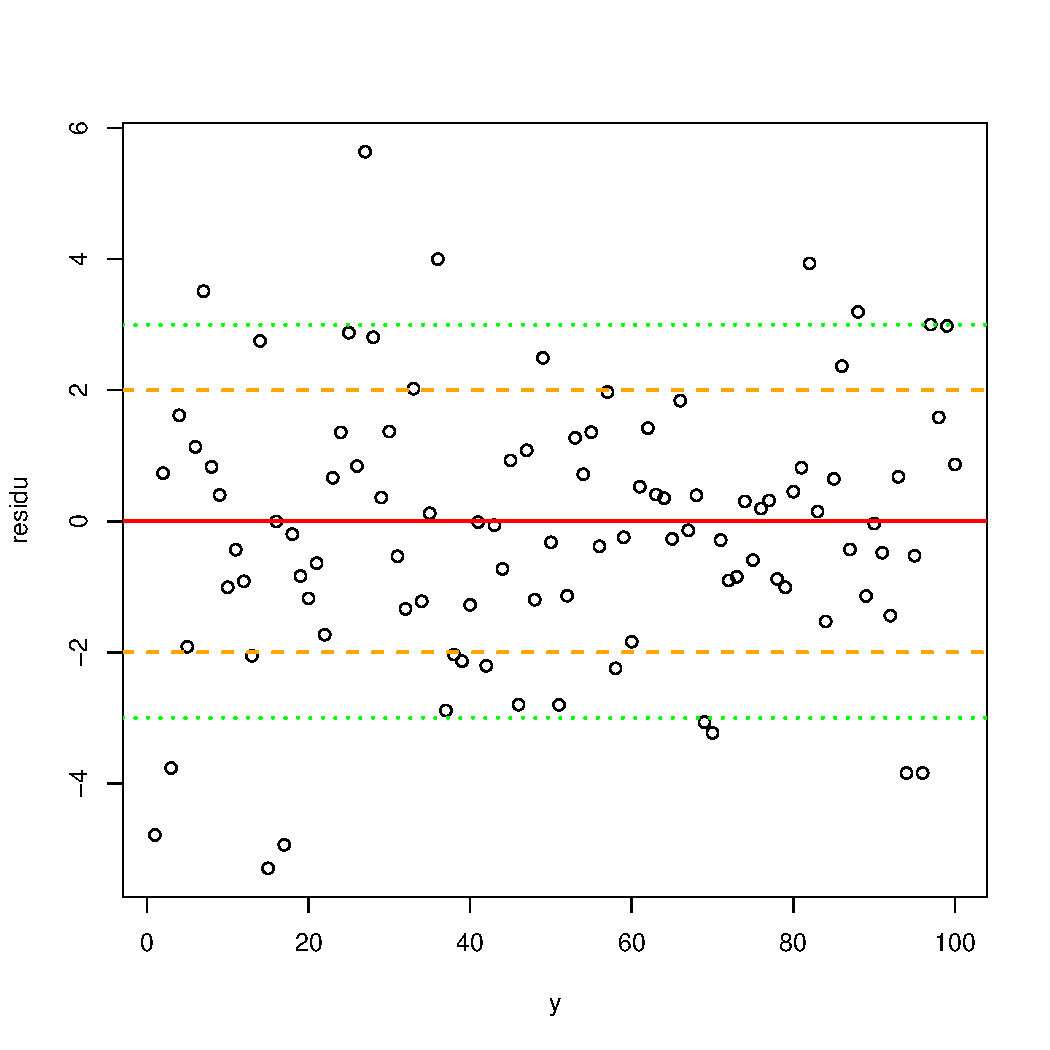
\includegraphics[width=.5\textwidth]{Img/reglin_residu_out}
  \begin{minipage}{.5\linewidth}
    \kern-.6\textheight
    \begin{itemize}
    \item résidus centrés et gaussiens
      \begin{itemize}
      \item moyenne nulle
      \item 95\% dans l'intervalle $\pm 2\sigma$
      \item 99\% dans l'intervalle $\pm 3\sigma$
      \end{itemize}
      \vfill

    \item détection des individus suspicieux (\emph{outliers})

    \item ces individus peuvent fausser la régression~!
    \end{itemize}
  \end{minipage}
}

%% =============================================================================
\subsection{Travaux pratiques}
% -----------------------------------------------------------------------------
\frame{%
  \frametitle{TP~: Qualité de la régression}
  \begin{enumerate}

    \bigskip
  \item Calculez le coefficient de corrélation linéaire (faire une fonction).

    \bigskip
  \item Calculez la variance totale, la variance expliquée, la
    variance résiduelle (faire des fonctions). Vérifiez la
    décomposition de la variance.

    \bigskip
  \item Calculez le coefficient de détermination (faire une fonction).

    \bigskip
  \item \emph{Astuce}~: savez-vous ajouter ces grandeurs sur le
    graphique (\texttt{text})~?
  \end{enumerate}
}

% -----------------------------------------------------------------------------
\frame{%
  \frametitle{TP~: Résidus}
  \begin{enumerate}

    \bigskip
  \item Tracez les résidus en fonction de $x$.
  \item Ces résidus vous semblent-ils «normaux»~? Y a-t-il des points
    suspicieux~?
    
    \bigskip

  \item Calculez la régression $y = a\,x^2 + b$.
  \item Est-elle meilleure~?
    \bigskip

  \item Parmi les régression de la forme $y = a\,x^k + b$, laquelle
    vous semble la meilleure~?
  \end{enumerate}
}

%% =============================================================================
\section[Rég. lin. multiple]{Régression linéaire multiple}
\subsection{Généralisation de la régression linéaire}
% -----------------------------------------------------------------------------
\frame{%
  \frametitle{TP~: \texttt{lm} (et \texttt{predict})}
  \begin{enumerate}

  \item Récupérez le fichier \texttt{003\_regression\_linaire\_lm.R}

  \item Exécutez-le pas à pas, en prenant le temps de comprendre
    chaque instruction proposée. 

    \bigskip
  \item Vérifiez que vous savez
    \begin{itemize}
    \item importer ou générer des données, tracer des graphiques pour
      les représenter~;
    \item calculer une régression linéaire avec une ou plusieurs
      variables, transformer les variables~;
    \item déterminer les caractéristiques essentielles d'une
      régression linéaire (coefficients, $R^2$, résidus, ...)~;
    \item calculer des prédictions pour les régressions calculées.
    \end{itemize}
  \end{enumerate}
}

% -----------------------------------------------------------------------------
\frame[allowframebreaks]{%
  \frametitle{Régression linéaire multiple}
  \begin{itemize}
  \item on étend la régression linéaire à $p$ variables explicatives
  \item on se limite à des fonctions linéaires (en chaque variable)
    
    \bigskip
    \begin{block}{Régression linéaire multiple}% Gaudoin, p27
      Le modèle de régression linéaire simple est défini par
      \[ y_i = \beta_p x_{p,i}  + \ldots + \beta_1 x_{1,i}  + \beta_0 + \epsilon_i, i=1..n\]
    \end{block}
    \begin{itemize}
    \item les $\beta_i$ sont les paramètres inconnus à estimer
    \item $\epsilon_i$ est le résidu pour l'observation $i$
    \end{itemize}

    \goodbreak

  \item hypothèse~: les résidus sont centrés
    \begin{itemize}
    \item si les résidus sont indépendants, de même loi et même
      variance $\sigma^2$, on parle de \alert{moindres carrées
        ordinaires}
    \item sinon on parle de \alert{moindres carrées généralisés}
    \end{itemize}
  \item il n'y a pas d'hypothèse sur les régresseurs (en particulier,
    ils n'ont pas à être indépendants)

    \bigskip
  \item écriture matricielle~: $\displaystyle Y = X \beta + \epsilon$ \\
    {\scriptsize
    \hfill%
    $Y = \left(\begin{array}{c}y_1\\\vdots\\y_n\end{array}\right)$
    \hfill%
    $X = \left(\begin{array}{cccc}
        1 & x_{11} &\ldots& x_{p1}\\
        \vdots & \vdots & \ddots & \vdots \\
        1 & x_{1n} &\ldots& x_{pn}\\
      \end{array}\right)$%
    \hfill%
    $\beta = \left(\begin{array}{c}\beta_0\\\vdots\\\beta_p\end{array}\right)$
    \hfill%
    $\epsilon = \left(\begin{array}{c}\epsilon_1\\\vdots\\\epsilon_n\end{array}\right)$}

  \end{itemize}
}

% -----------------------------------------------------------------------------
\frame{%
  \frametitle{Calcul des paramètres}% Gaudoin, p29
  \begin{itemize}
  \item on veut minimiser l'erreur quadratique (moyenne)~: $||Y -
    X\beta||_2$

    \vfill
  \item dans le cas des moindres carrés ordinaires $\beta$ minimise
    $||Y - X\beta||_2$ ssi
    \[ X^TX\beta = X^TY \] («équations normales» de la régression
    linéaires)
    \vfill
  \item dans le cas des moindres carrés généralisés, il faut faire des
    hypothèses sur les résidus...
  \end{itemize}
}

% -----------------------------------------------------------------------------
\frame{%
  \frametitle{Coefficients de corrélation linéaire}
  \begin{itemize}
  \item[]
    \begin{block}{Coefficient de corrélation}% Gaudoin, p42
      Le coefficient de corrélation linéaire multiple entre la
      variable à expliquer $y$ et les régresseurs $x_i$ est
      \[r = \sup_{a_1,...,a_p} r_{y,\sum a_jx_j}\]
    \end{block}
    \begin{itemize}\scriptsize
    \item $r$ est la valeur maximale prise par le coefficient de
      corrélation linéaire entre $y$ et une combinaison linéaire des $x_j$.
    \item $r\in[0;1]$
    \end{itemize}
    
    \vfill
  \item conséquence de la définition~: \alert{ajouter des variables
      augmente $r$} \\ (sauf colinéarité)
  \end{itemize}
}

% -----------------------------------------------------------------------------
\frame{%
  \frametitle{Coefficient de détermination}% Gaudoin p42
  \begin{itemize}
  \item[]
    \begin{block}{Coefficient de détermination}
      Le coefficient de détermination de la régression linéaire
      est \[R^2 = \frac{SSR}{SST} = 1 - \frac{SSE}{SST}\]
    \end{block}\kern-5mm
  \item identique à la régression linéaire simple
  \item «\emph{multiple R-squared}» sous \texttt{R}
    \vfill
  \item propriété~: $R^2 = r^2$ \\
    corollaire~: $R^2$ augmente avec le nombre de variables...
  \end{itemize}
}

% -----------------------------------------------------------------------------
\frame{%
  \frametitle{Coefficient de détermination ajusté}
  % http://en.wikipedia.org/wiki/Coefficient_of_determination  !! er form R2_adj (2ème partie de la formule)
  \begin{itemize}
  \item enjeux~:
    \begin{itemize}
    \item maximiser $R^2$ n'est pas un bon critère de qualité, car
      ajouter des variables aléatoires serait «bénéfique»
    \item on ne peut pas comparer deux modèles avec un nombre de
      variables différent
    \end{itemize}
    \vfill
  \item idée~: pénaliser le $R^2$ en fonction du nombre de variables

  \item[]
    \begin{block}{Coefficient de détermination ajusté}
      Le coefficient de détermination ajusté de la régression linéaire
      est \[R^2_{adj} = 1 - (1-R^2)\frac{n-1}{n-p-1}\]
    \end{block}
    \begin{itemize}\scriptsize
    \item $n-1$ : degrés de liberté de SST
    \item $n-p-1$ : degrés de liberté de SSE
    \end{itemize}

  \end{itemize}
}

% -----------------------------------------------------------------------------
\frame{%
  \frametitle{Conclusion partielle}
  \begin{itemize}
  \item nous savons calculer des modèles de régression linéaire
  \item nous savon évaluer ces modèles, dans une certaine mesure
    \vfill
  \item encore beaucoup à dire sur la construction et l'interprétation de modèles linéaires
    \begin{itemize}
    \item autres critères de qualité (que le $R^2_{adj}$)
    \item tests statistiques sur la significativité d'une variable
    \item méthodes de construction et de sélection des variables
    \item analyse des erreurs, intervalles de confiance des prédictions
    \item ...
    \end{itemize}
  \end{itemize}
}

\subsection{Travaux pratiques}
% -----------------------------------------------------------------------------
\frame[allowframebreaks]{%
  \frametitle{TP~: Consommation de véhicules}

  Jeu de données \texttt{mpg.dat}
  (\href{http://archive.ics.uci.edu/ml/datasets/Auto+MPG}{UCI Machine
    Learning Repository})~:% avec 392 voitures~:
  \begin{itemize}
  \item \texttt{mpg} (\textit{miles per galon})~: la distance
    parcourue %(miles/galon)% d'essence consommée, en cycle urbain.
  \item \texttt{cylinders}~: le nombre de cylindres.
  \item \texttt{displacement} (pouces-cube)~: la cylindrée% (pouces-cubes)
    %c'est-à-dire le volume déplacé par les pistons des cylindres.
  \item \texttt{horsepower}~: puissance du moteur 
  \item \texttt{weight} (livres)~: poids du véhicule%, vraissemblablement en livres.
  \item \texttt{acceleration}~: secondes pour atteindre 100 m/h
    %vraissemblablement exprimée comme le temps (en seconde) pour
    %atteindre les 100 miles par heure.
  \item \texttt{model year}~: année du modèle.
  \item \texttt{origin}~: lieu (1~-~USA~; 2~-~EU~; 3~-~Japon).
  \item \texttt{name}~: nom du modèle (unique).
  \end{itemize}

  \goodbreak

  TP noté~!
  \begin{itemize}
  \item à faire en binôme.
  \item à rendre sur Chamilo le dimanche 6 mars 2016.
  \item rendu~: script R \alert{commenté}.
    \begin{itemize}
    \item Les commandes permettant de répondre à une question doivent
      être fournies, à l'exclusion de toutes autres.
    \item Les graphiques doivent être soignés, clairs et complets.
    \item Une réponse explicite, pour chaque question, est
      requise. Cette réponse sera rédigée convenablement (hormis
      fonctions ou graphiques demandés).
    \end{itemize}
  \end{itemize}
}

\end{document}


% -----------------------------------------------------------------------------
\frame{%
  \frametitle{Intervalles de confiance}
  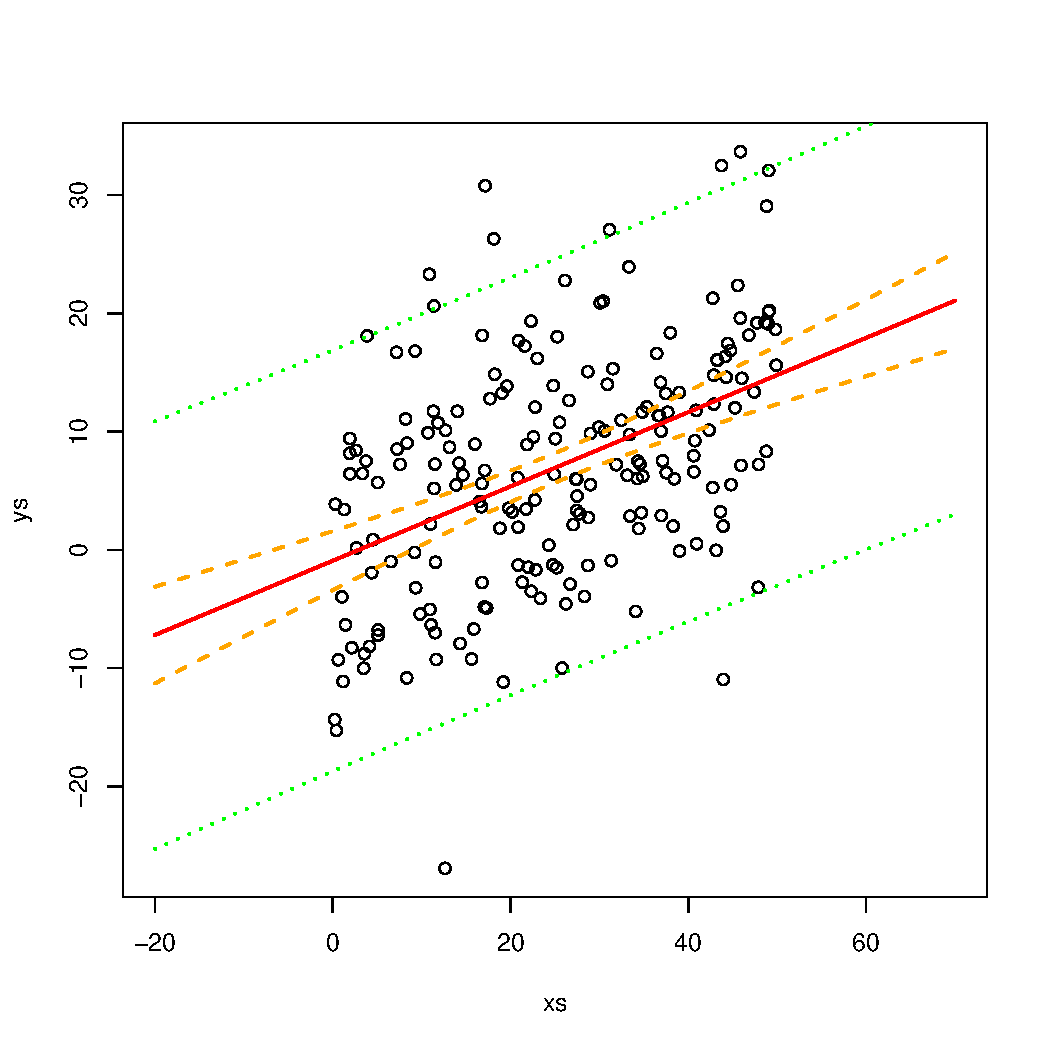
\includegraphics[height=\textheight,width=.7\textwidth]{Img/reglin_intervalles}
  \kern-5mm
  \begin{minipage}{.3\linewidth}
    \kern-\textheight
    \begin{itemize}
    \item intervalle pour la moyenne des prédictions
    \item intervalle pour une prédiction individuelle
    \item hypothèses de validité de ces intervalles
    \item limites de validité du modèle
    \end{itemize}
  \end{minipage}
  %
  \IGNORE{%
    pdf("reglin_intervalles.pdf")
    xs <- runif(n=200, min=0, max=50)
    ys <- 0.25*xs + 2 + rnorm(n=length(xs), mean=0, sd=10)
    ds <- data.frame(cbind(ys,xs))
    m <- lm(ys ~ xs, data=ds)
    plot(ys ~ xs, data=ds, xlim=c(-20,70))

    xs <- -20:70 ; ds <- data.frame(xs)
    matlines(xs, predict(m,ds, interval="conf"), lty=c(1,2,2), col=c("red", "orange", "orange"), lw=2)
    matlines(xs, predict(m,ds, interval="prediction"), lty=c(1,3,3), col=c("red", "green", "green"), lw=2)
    dev.off()

  }
}

% =============================================================================
% =============================================================================
\subsection{Régression linéaire multiple}

% -----------------------------------------------------------------------------
\frame<handout:0>{%
  \begin{block}{Travaux pratiques} question 22
  \end{block}
  \begin{itemize}
  \item ...
  \end{itemize}
}

% -----------------------------------------------------------------------------
\frame{%
  \frametitle{Influence des variables}%
  \begin{itemize}
  \item le signe d'une variable indique le sens de l'effet
  \item le coefficient d'une variable indique son apport
    \vfill
    \begin{center}
      \alert{ATTENTION}
    \end{center}
  \item \alert{l'interprétation des coefficients doit tenir compte des unités} \\
    {\scriptsize passer un poids de kg à g multiple les coefficients
      par 1000, sans en changer l'importance}
  \item \alert{l'interprétation des coefficients doit tenir compte des variances} \\
    {\scriptsize un grand coefficient pour une variable qui ne varie
      pas est ... une constante}
  \item \alert{les coefficients (et signes) sont biaisés par les dépendances} \\
    {\scriptsize en cas de colinéarité, une infinité de coefficients
      existent, celui d'une variable venant corriger celui de l'autre
      variable}
  \item \alert{les coefficients ne sont pas tous significatifs} \\
    {\scriptsize il existe des tests statistiques pour cela ... voir
      les \texttt{*} de \texttt{R}}

  \end{itemize}
}

% -----------------------------------------------------------------------------
\frame{%
  \frametitle{Variables artificielles}%
  \begin{itemize}
  \item on peut «construire» toutes les variables que l'on veut
  \item infinité de transformations et de combinaisons !
    \vfill
  \item utiliser la connaissance \emph{a priori} du problème
    (influence des paramètres, relations entre paramètres)
  \item étudier les résidus en fonction des différentes variables déjà
    identifiées
  \end{itemize}
}

% -----------------------------------------------------------------------------
\frame{%
  \frametitle{Sélection de variables (1)}%
  \begin{itemize}
  \item déterminer l'enjeu~:
    \begin{itemize}
    \item trouver la meilleure représentation des données~?
    \item trouver le meilleur modèle pour faire des prédictions~?
    \item déterminer si une variable est importante~?
    \item ...
    \end{itemize}
    \vfill
  \item en déduire les modes d'évaluation
    \begin{itemize}
    \item critères~: $R^2_{adj}$, erreur moyenne, erreur relative, ...
    \item différence de qualité par rapport modèles de référence
    \item validation croisée ou non
    \end{itemize}
  \end{itemize}
}

% -----------------------------------------------------------------------------
\frame{%
  \frametitle{Sélection de variables (2)}%
  \begin{itemize}
  \item méthode exhaustive~: tester tous les sous-ensembles~!
    \begin{itemize}
    \item $p$ variables $\implies$ $2^p$ sous-ensembles ... \\
      {\scriptsize avec 1000 sous-ensembles/sec, il faut plus d'une
        heure pour 22 variables, plus d'un jour pour 27 variables,
        plus d'un an pour 35 variables}
    \end{itemize}
    \vfill
  \item méthode «métier»~: tester les sous-ensembles ayant une
    signification particulière
    \vfill
  \item méthodes heuristiques
    \begin{itemize}
    \item tri des variables par corrélation avec $y$, et ajout dans cet ordre (bof)
    \item à chaque itération, ajouter la variable la mieux corrélée
      aux résidus
    \item à chaque itération, on essaie d'enlever ou d'ajouter chacune
      des variables (donc $p$ modèles à chaque itération)
    \end{itemize}


  \end{itemize}
}

% -----------------------------------------------------------------------------
\frame<handout:0>{%
  \begin{block}{Travaux pratiques} reprendre question 22
  \end{block}
  \begin{itemize}
  \item \texttt{m <- lm(mpg \string~ ., data=mpg)} \\
    \texttt{step(m, direction="both")~~~~~\# critère AIC}
  \item \texttt{library(leaps)}\\
    \texttt{selm <- regsubsets(mpg \string~ . - name, data=mpg)}\\
    \texttt{plot(selm, scale="bic")~~~~~~~\# critère BIC}\\
    \texttt{plot(selm, scale="adjr2")~~~~~\# critère $R^2_{adj}$}
  \end{itemize}
}

% -----------------------------------------------------------------------------
\frame{%
}

\end{document}
